\documentclass[10pt,a4paper,notitlepage]{article}
\usepackage[utf8]{inputenc}
\usepackage[T1]{fontenc}
\usepackage{amsmath}
\usepackage{amsfonts}
\usepackage{amssymb}
\usepackage{array}
\usepackage{float}
\usepackage{graphicx}
\usepackage{subcaption}
\usepackage{float}
\begin{document}
\title{Project CFD--Lab\\ \textit{Free Surface Simulation}}
\author{\textbf{Group Number : 1}\\Krenz Lukas Reiser Andreas Kouroudis Ioannis \\ \\\textbf{Supervisor}\\Menhorn Friedrich }
\maketitle
\section*{Abstract}
In industry there are many applications that require the simulation of a system of unmixable fluids with vastly different kinematic viscosity, separated by a discrete interface.  This problem is commonly referred to as a free surface flow problem. In effect, the kinematic viscosity difference causes the first fluid, which is usually the industrially relevant one, to exert force on the second one, receiving a negligible reaction in return. The most common configuration of this sort is a liquid-gas system and is frequently encountered in applications such as dam breaking scenarios, material processes and wave simulations.

	In this particular project, the phenomenon is simulated  using a Lattice Boltzmann approach combined with volume of fluid method. To track the interface, the mass streamed in and out of the interface cells is calculated. We consider filled cells to have a volume equal to 1 and empty cells equal to 0. When a cell emptied, all the neighboring fluid cells became interface cells. Equally, when an interface cell was filled, all the neighboring empty cells became interface cells.
	The program was written in C\texttt{++} utilizing omp parallelization.
\\
\section{Aspects of implementation}
\subsection{Boundary conditions}
In addition to the previously implemented boundary conditions (Free slip, No slip, , etc) a new condition was implemented, namely a free surface boundary condition.
The physical perspective of this condition is that the gas has a far greater kinematic viscosity and is consequently pushed without resistance by the liquid. Further, it is assumed that the gas pressure is atmospheric, which is used in place of density in the equilibrium function($\rho_{A} = 1$).
If $e_{i}$ from an interface cell points to an empty cell the following distribution is constructed:
\begin{equation} \label{eq:dist}
f'_{\hat{i}} (x, t + \Delta t) = f^{eq}_{\hat{i}}(1, \mathbf{u})+f^{eq}_{{i}}(1, \mathbf{u})-f_{i}(\mathbf{x},t)
\end{equation}

However, constructing these distributions along only one side of the interface would result in a force imbalance. To rectify this, additional distributions have to be reconstructed during the streaming step.

If $\mathbf(n*e_{i})>0$
$f_{i}$ is reconstructed according to equation \eqref{eq:dist}

n is the vector normal to the interface and is computed as the central differences of the fluid fraction between neighboring cells
\begin{equation} \label{eq:normal}
\mathbf{n}=\frac{1}{2}\begin{bmatrix} \epsilon(x_{j-1,k,l})-\epsilon(x_{j+1,k,l})\\\epsilon(x_{j,k-1,l})-\epsilon(x_{j,k+1,l})\\\epsilon(x_{j,k,l-1})-\epsilon(x_{j,k,l+1} ) \end{bmatrix}
\end{equation}

\subsection{gravity }
As in our scenarios there is need of an accelerating force (gravity) the BGK lattice Boltzmann equation is transform according to \eqref{eq:BGK}\cite{thurey2006optimization}
\begin{equation} \label{eq:BGK}
f_{i}(x,t+\Delta t)=(1-\omega)f_{i}^{eq}+\omega f_{i}^{eq}(\rho(\mathbf{x},t),\mathbf{u}(\mathbf{x},t)+\frac{g}{\omega})
\end{equation}
\subsection{Mass exchange}
In order to keep track of the interface two additional variables have to be stored for each cell, namely mass m and the density $\rho$. The mass exchanged between an interface and a fluid cell  is found directly using their distributions. 
\begin{equation} \label{eq:fluid-interface}
\Delta m_{i}(x,t+\Delta t)=f_{\hat{i}}(x+e_{i},t)-f_{i}(x,t)
\end{equation}

For interface-fluid cell the mass exchange must take into account the interface shared between them. During this step, there might still remain interface cells amidst either fluid or empty cells. These artifacts are corrected using the equation \eqref{eq:intint} in conjucture with the table \ref{table:artifacts}. Since the mass lost from one cell is the mass gained from another, the mass exchange is a symmetric process.
\begin{equation} \label{eq:intint}
\Delta m_{i}(x,t+\Delta t)=s_{e} \frac{e(x+\Delta t*e_{i},t)+e(x,t)}{2}
\end{equation}

\begin{table}[H]
\centering
\label{table:artifacts}
\begin{tabular}{lllll}
 		&  standard cell at $(x+e_{i})$	& no fluid nb at $(x+e_{i})$     & no empty nb at $(x+e_{i})$    \\
 standard cell at (x)		&$f_{\hat{i}}(x_{nb},t)-f(x,t)$	&  $f_{\hat{i}}(x_{nb},t)$		&$-f_{i}(x,t)$		    \\
 no fluid neighbors at $(x)$	&$-f_{i}(x,t)$			&  $f_{\hat{i}}(x_{nb},t)-f(x,t)$	&$-f_{i}(x,t)$		     \\
 no empty neighbors at $(x)$	&$f_{\hat{i}}(x_{nb},t)$	&  $f_{\hat{i}}(x_{nb},t)$		&$f_{\hat{i}}(x_{nb},t)-f(x,t)$
\end{tabular}
\caption{Interface Interface mass streaming $s_{e}$ coefficient}
\end{table}

\subsection{Flag Update}
After the mass calculation step, all the interface cells that have a density higher than 1 are assigned a temporal flag as Fluid cells, and their surrounding Empty cells become interface. Following the same principle, all previously interface cells with mass lesser or equal to zero become empty cells, and their surrounding fluid cells recieve a temporal interface cell flag. The temporal flag serves to make the update order independent. As the former empty cells become interface they are initialised with the average density and velocity of their surrounding cells, excluding empty ones, which would otherwise be included if the update was made at this point. In practice, to avoid constant emptying and filling of cells when they are close to changing their state, a tolerated offset is introduced, transforming the criterion in the following fashion.

\begin{equation} \label{eq:filled}
M(x,t+ \Delta t)>(1+offset)*\rho(x,t+\Delta t)
\end{equation}
\begin{equation} \label{eq:empty}
M(x,t+ \Delta t)<(0-offset)*\rho(x,t+\Delta t)
\end{equation}
In this case the used offset was $10^{-3}$\cite{thurey2007physically}. Formerly empty cells that become interface cells are initialised with the average density and velocity of their surrounding cells.
\subsection{Excess Mass }

After the flagfield has been updated, excess or negative mass issues are tackled. All newly empty or filled cells possibly have mass greater than 1 or lesser than 0. This is corrected by distributing or taking mass from the nearby interface cells. The distribution is weighted according to the relative position of the cell direction to the normal vector of the current cell. Specifically:
\begin{equation} \label{eq:exmass}
\Delta m(x+e_{i})=m^{ex}\frac{v_{i}}{v_{total}}
\end{equation}
Where $v_{total}$ is the sum of all weights and $v_{i}$ is the weight of the neighboring cell calculated as follows:

for filled cells:
\begin{equation} \label{eq:filledweight}
  v_i = 
  \begin{cases}
    \mathbf{n*e_{i}}     & \quad \text{if }  \text{$\mathbf{n*e_{i}}>0$}\\
    0			 & \quad \text{if }  \text{otherwise}\\
  \end{cases}
\end{equation}

for empty cells
\begin{equation} \label{eq:emptyweight}
  v_i = 
  \begin{cases}
    -\mathbf{n*e_{i}}     & \quad \text{if }  \text{$\mathbf{n*e_{i}}<0$}\\
    0			  & \quad \text{if }  \text{otherwise}\\
  \end{cases}
\end{equation}

\subsection{Adaptive time step and turbulent model}

To avoid instabilities and to acquire speedup during periods of rest an adaptive time step was used. If $|u_{max}|>\frac{5}{24}$ the new timestep becomes $\Delta t_{n}=\frac{4}{5}*\Delta t_{old}$
Consequently, all time related quantities must be updated as well to keep the particle distributions inside either the current or the neigbouring cells over the course of one time iteration. This is done according to the following equations:
\begin{equation} \label{eq:dt}
s=\frac{\Delta t_{n}}{\Delta t_{o}}
\end{equation}
\begin{equation} \label{eq:omega}
\omega=\frac{1}{s(\frac{1}{\omega_{o}}-\frac{1}{2})+\frac{1}{2}}
\end{equation}
\begin{equation} \label{eq:density}
\rho_{n}=s(\rho_{o}-\rho_{med})+\rho_{med}
\end{equation}
\begin{equation} \label{eq:velocity}
u_{n}=su_{o}
\end{equation}
\begin{equation} \label{eq:gravity}
g=s^{2}*g_{o}
\end{equation}

Time steps can also increase in periods of relative calmness.If $|u_{max}|<\frac{1}{6}*\frac{5}{4}$ the resize factor is $\frac{5}{4}$. The logic behind $\frac{1}{6}$ is that it is half the speed of sound. If a velocity increases beyond this threshold, $f^{eq}$ will become negative.
If $\omega<1.99$, as this will cause negative equilibrium distributions and numerical instabilities. Some of the simulated scenarios generated a high degree of turbulence and quickly became unstable. To rectify this, a turbulence model was introduced. The local stress tensor is computed and subsequently used to modify the relaxation time according to the eddy viscosity. The Smagorinsky constant C is set to 0.03 \cite{thurey2007physically}. The non equilibrium stress tensor $\Pi_{\alpha\beta}$ is computed according to the equation \eqref{eq:stress}

\begin{equation} \label{eq:stress}
\Pi_{\alpha,\beta}=\sum^{19}_{i=1}e_{i\alpha}e_{i\beta}(f_{i}-f_{i}^{eq})
\end{equation}
where $\alpha$ and $\beta$ run over the three spatial direction
 The intensity of the local stress tensor S is computed as 
\begin{equation} \label{eq:intensity}
S=\frac{1}{6C^{2}}(\sqrt{\nu^{2}+18C^{2}\sqrt{\sum^{3}_{\alpha=1}\sum^{3}_{\beta=1}\Pi_{\alpha,\beta}^{2}}-\nu}
\end{equation}
and the modified relaxation time is given according to \eqref{eq:relax}

\begin{equation} \label{eq:relax}
\tau_s=3(\nu+C^{2}S)+\frac{1}{2}
\end{equation}
\section{Results/Scenario}
Two simple scenarios were chosen, and as can be seen produced very good physical results.
\subsection{Dam Breaking}
The dam breaking was simulated by having a large vertical mass of fluid at the start be released for one side of the geometry.
\begin{figure}[H]
\centering
\begin{subfigure}{0.25\textwidth}
  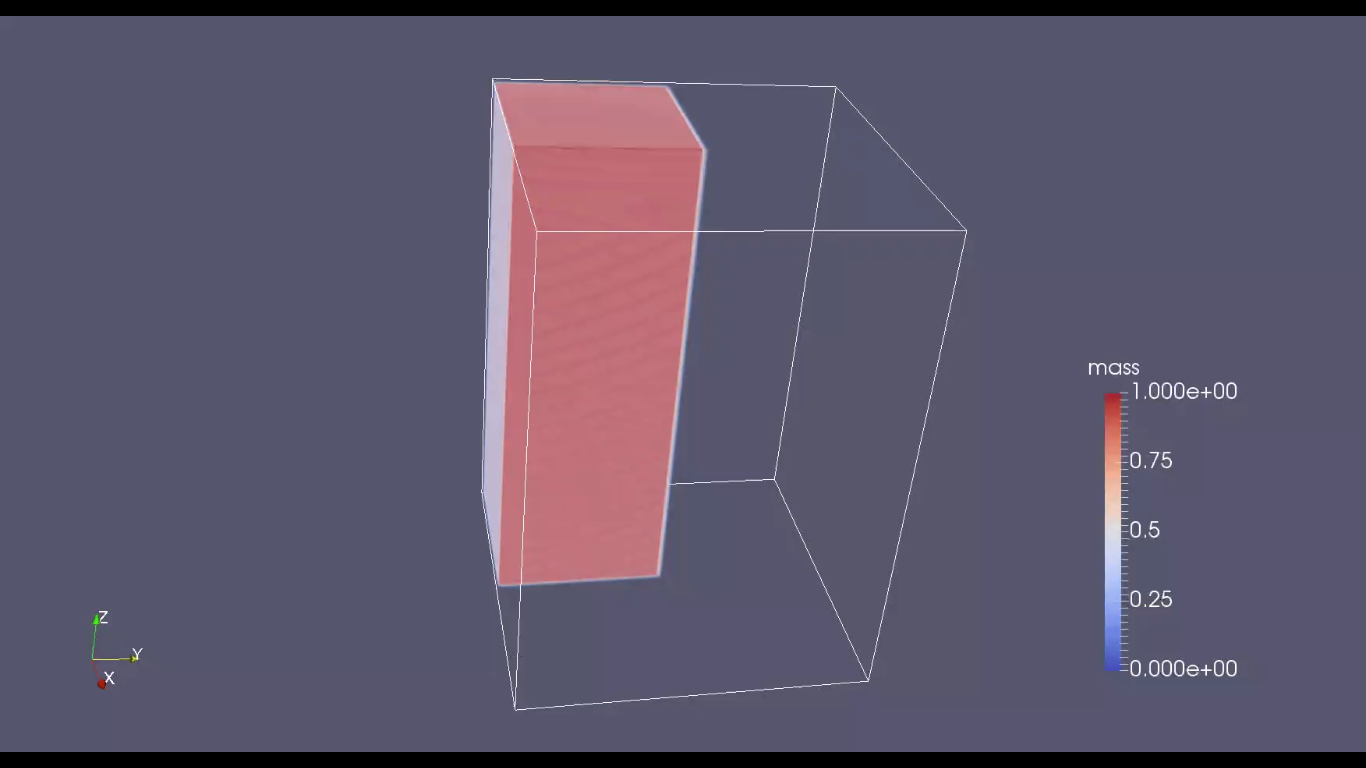
\includegraphics[width=1.0\linewidth]{dam/1.png}
\end{subfigure}%
\begin{subfigure}{0.25\textwidth}
  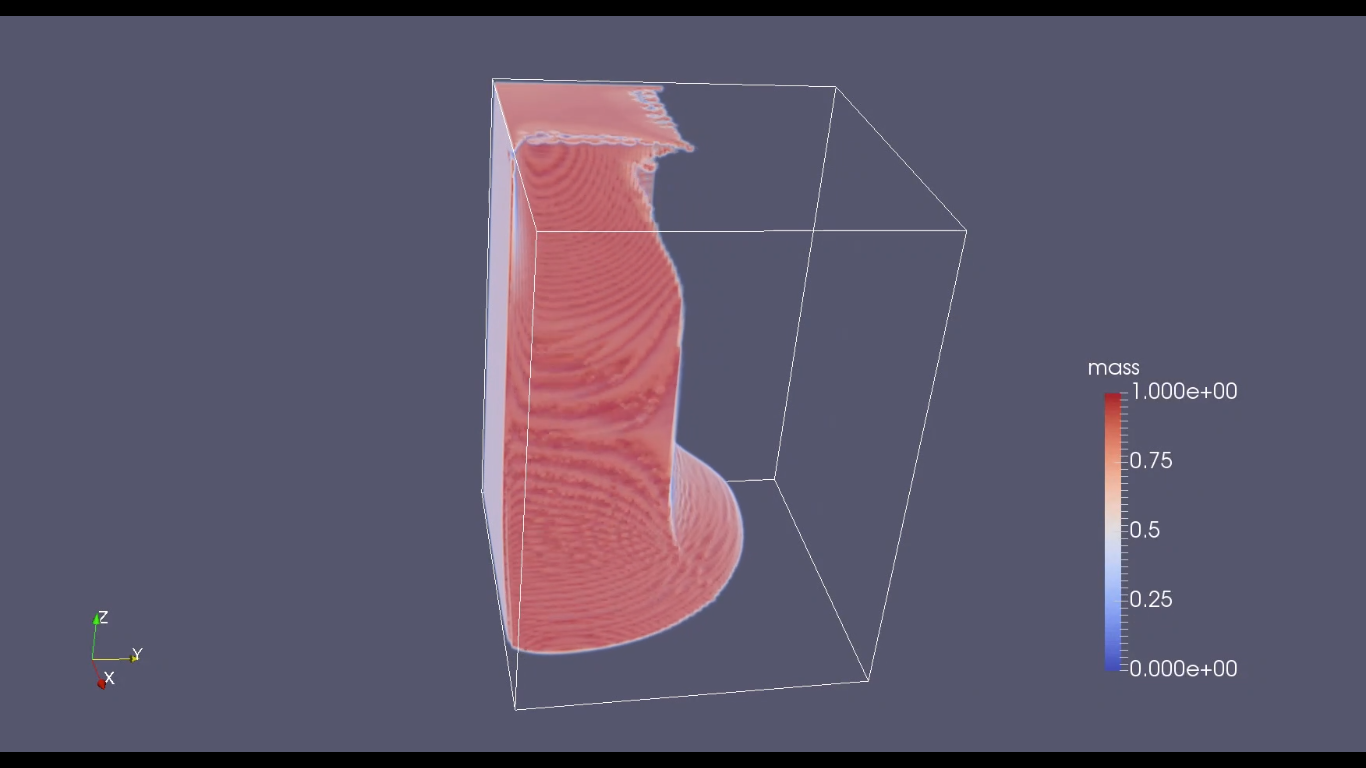
\includegraphics[width=1.0\linewidth]{dam/2.png}
\end{subfigure}
\begin{subfigure}{0.25\textwidth}
  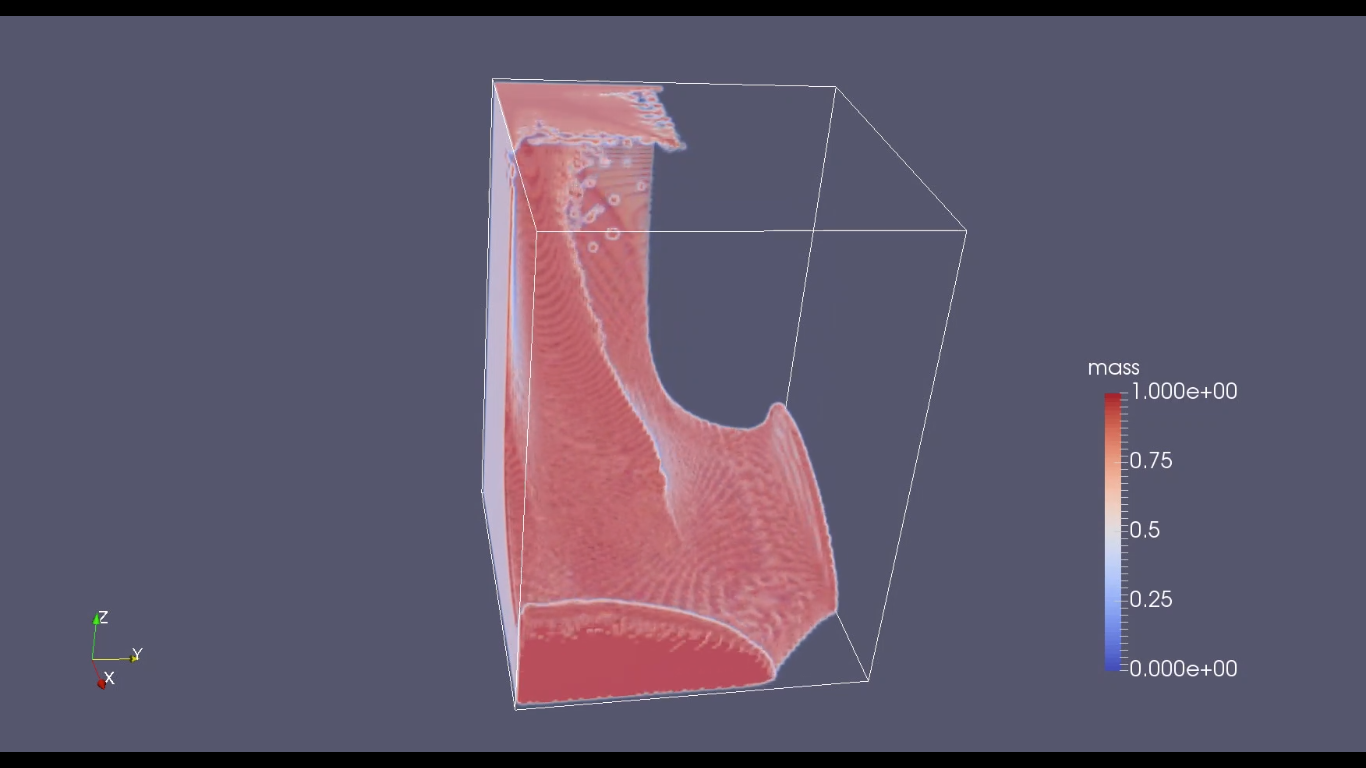
\includegraphics[width=1.0\linewidth]{dam/3.png}
\end{subfigure}
\centering
\begin{subfigure}{0.25\textwidth}
  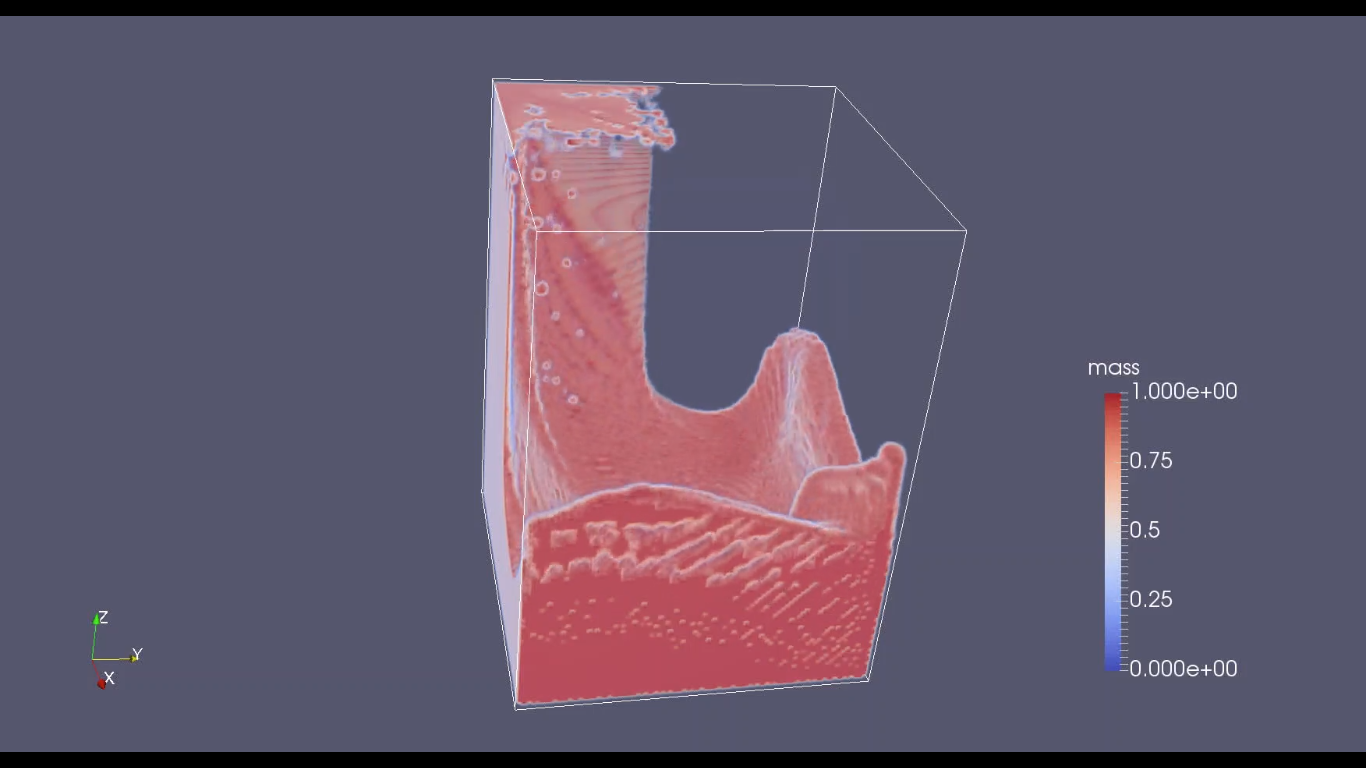
\includegraphics[width=1.0\linewidth]{dam/4.png}
\end{subfigure}%
\begin{subfigure}{0.25\textwidth}
  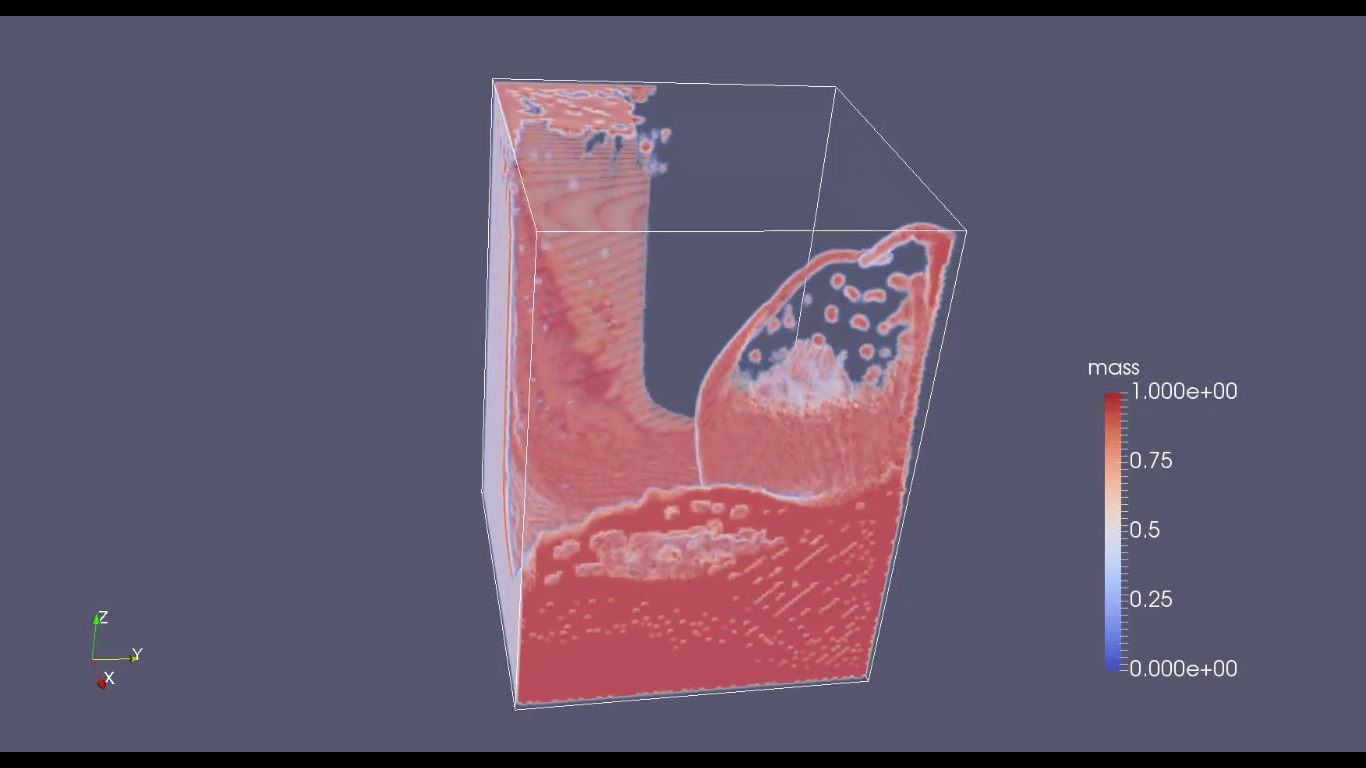
\includegraphics[width=1.0\linewidth]{dam/5.png}
\end{subfigure}
\begin{subfigure}{0.25\textwidth}
  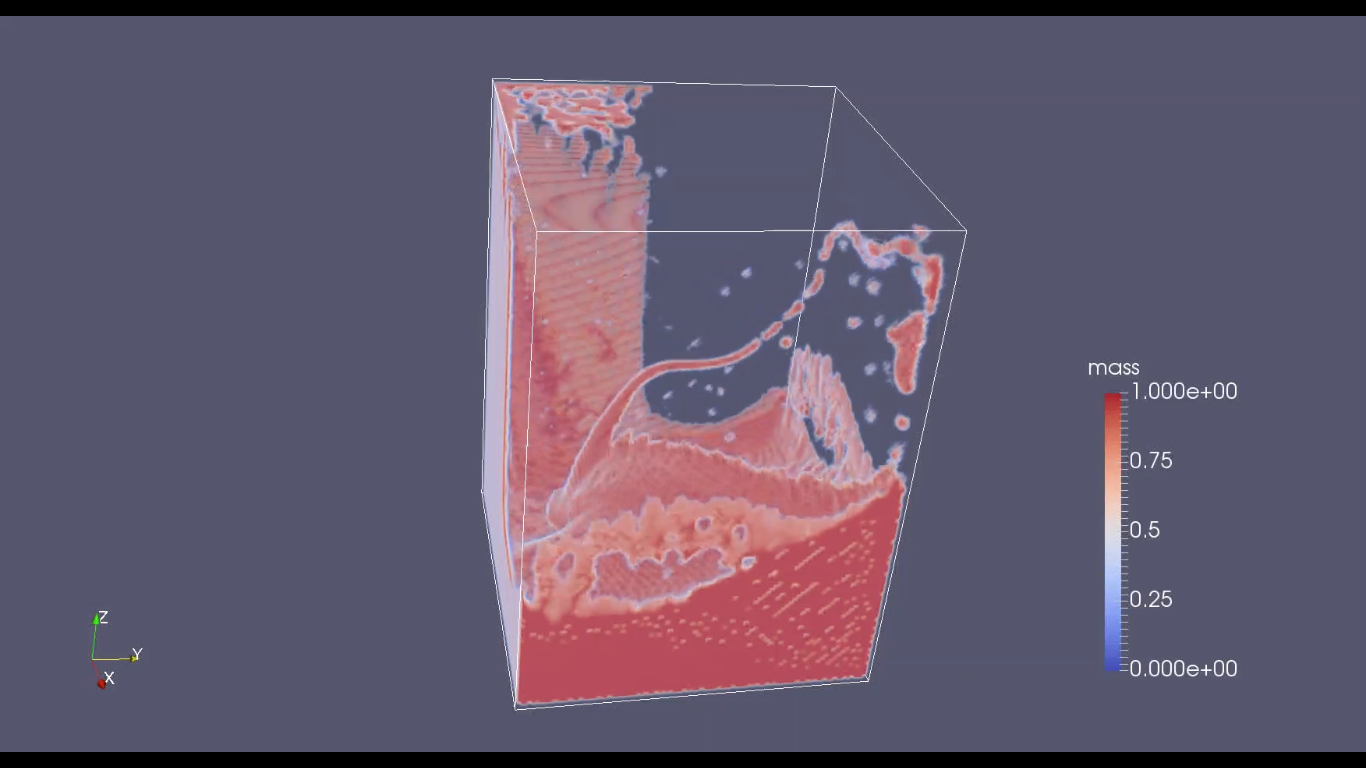
\includegraphics[width=1.0\linewidth]{dam/6.png}
\end{subfigure}
\centering
\begin{subfigure}{0.25\textwidth}
  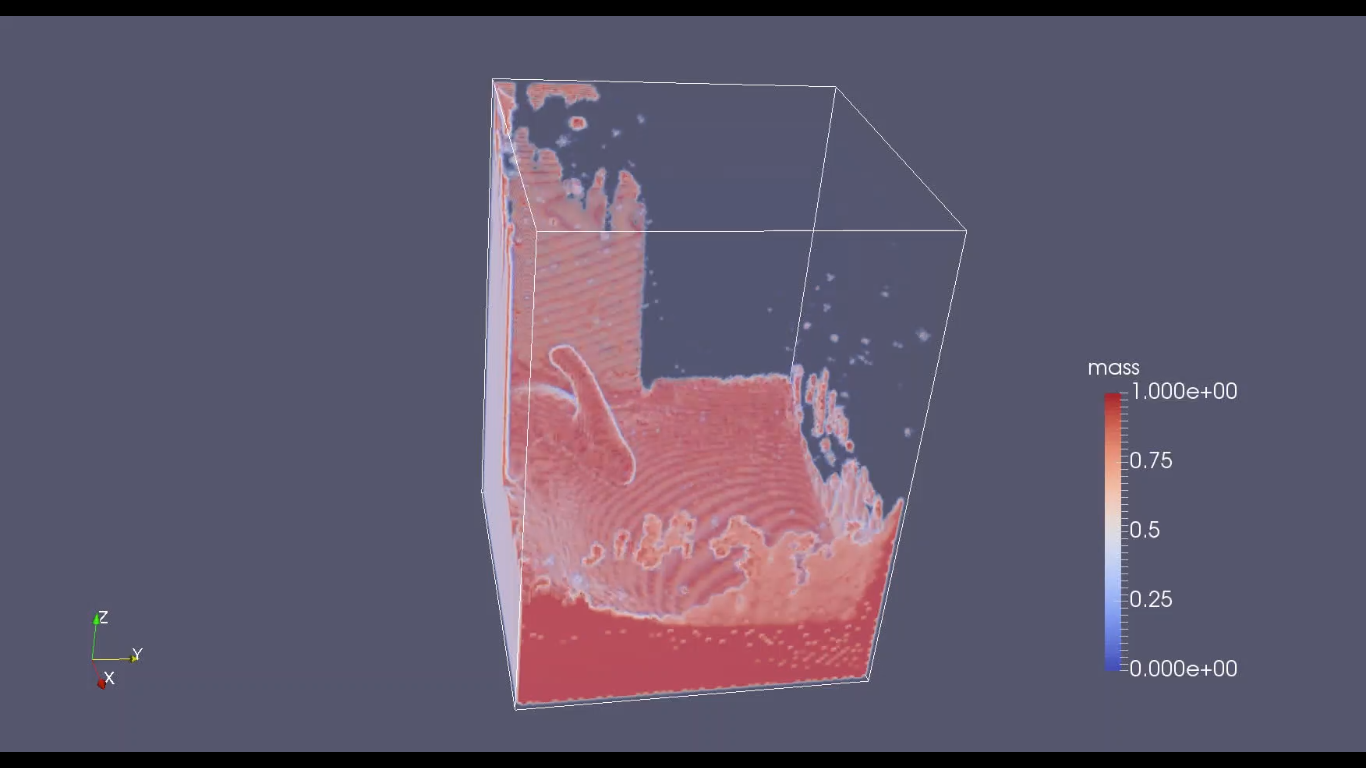
\includegraphics[width=1.0\linewidth]{dam/7.png}
\end{subfigure}%
\begin{subfigure}{0.25\textwidth}
  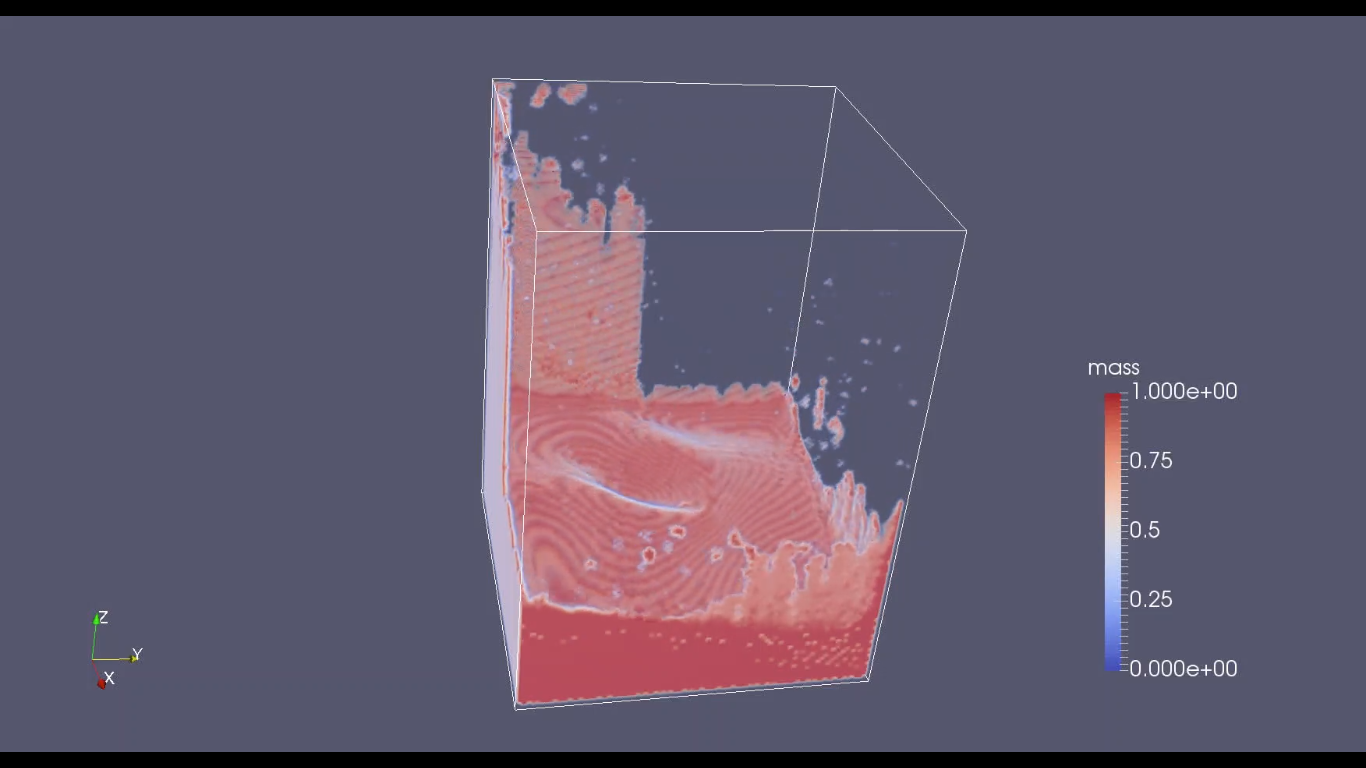
\includegraphics[width=1.0\linewidth]{dam/8.png}
\end{subfigure}
\begin{subfigure}{0.25\textwidth}
  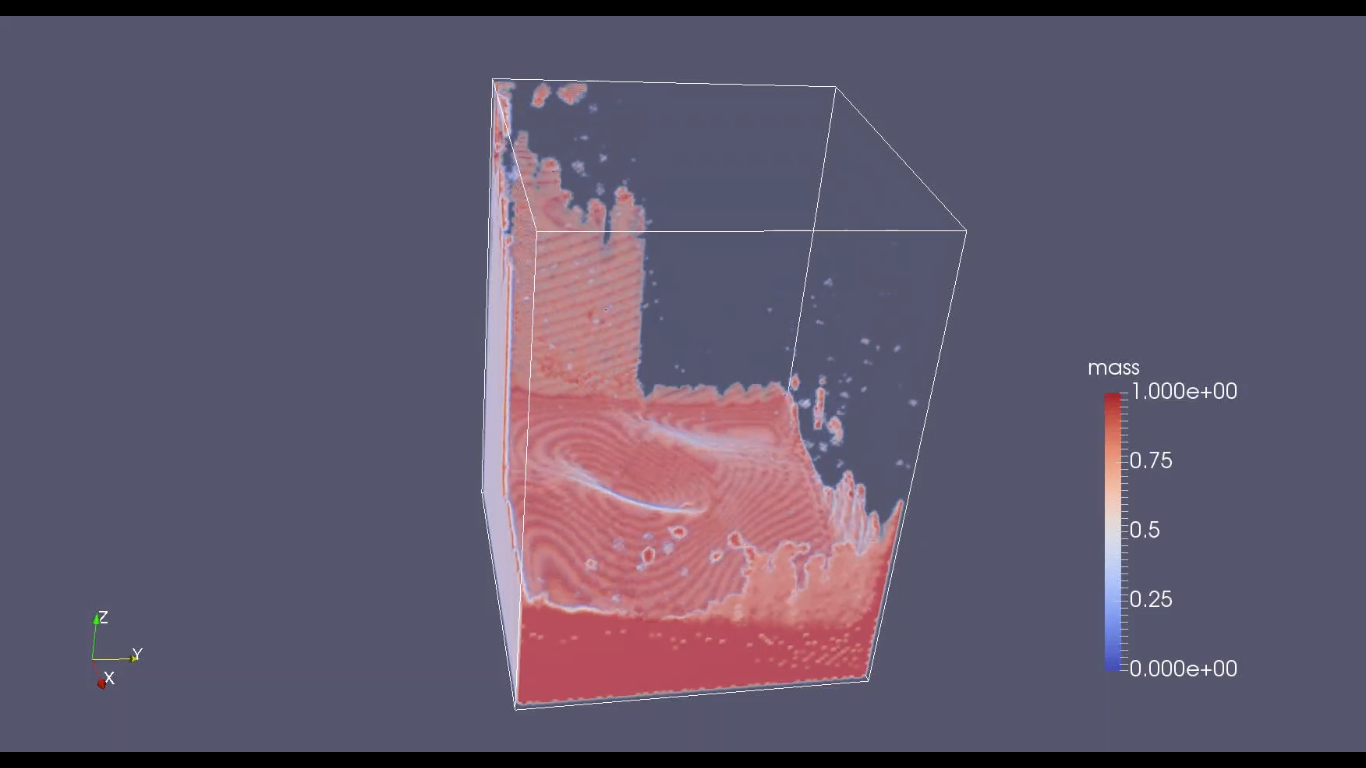
\includegraphics[width=1.0\linewidth]{dam/9.png}
\end{subfigure}
\caption{Breaking Dam}
\label{fig:dam}
\end{figure}
\subsection{Falling Drop}
A drop was left to fall in a pool of stationary water. As can be seen, the results look comparable to other sources and resemble the expected physical behaviour.
\begin{figure}[H]
\centering
\begin{subfigure}{0.25\textwidth}
  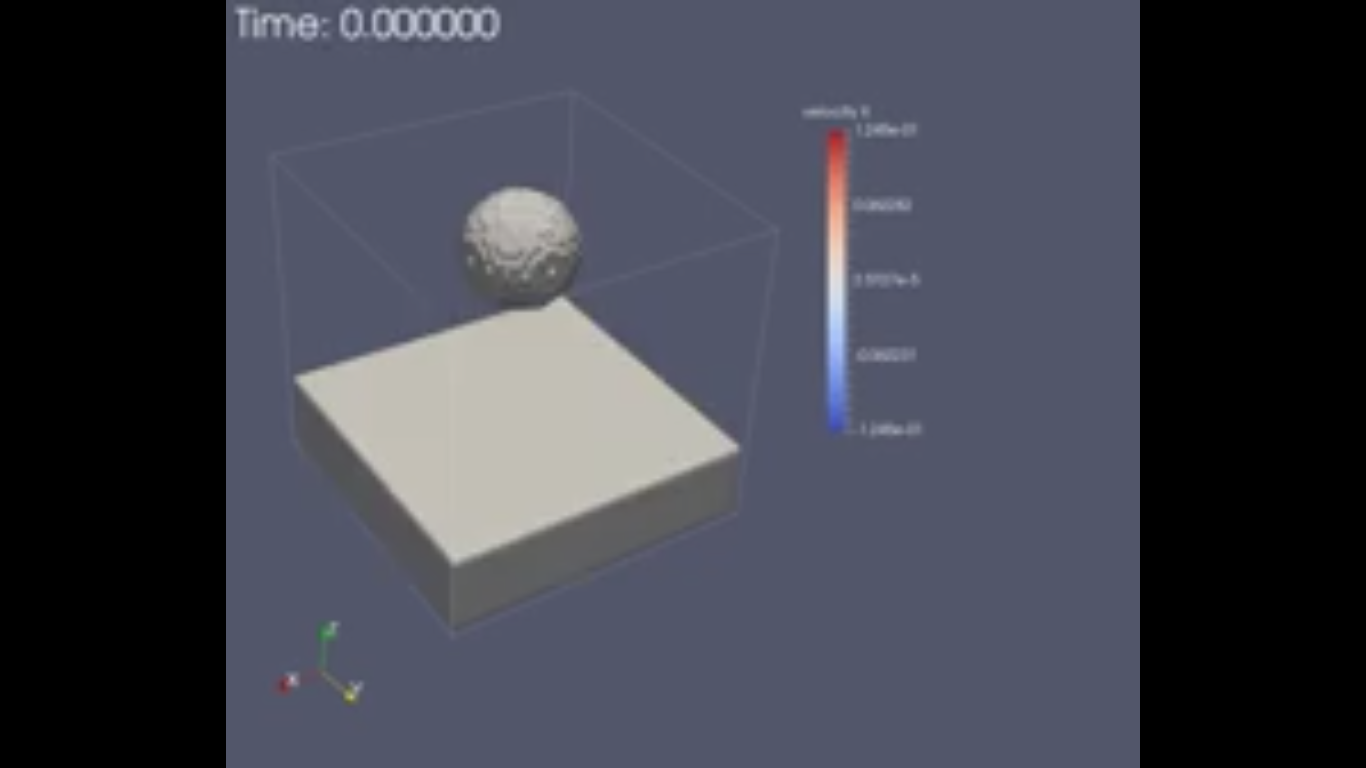
\includegraphics[width=1.0\linewidth]{drop/1.png}
\end{subfigure}%
\begin{subfigure}{0.25\textwidth}
  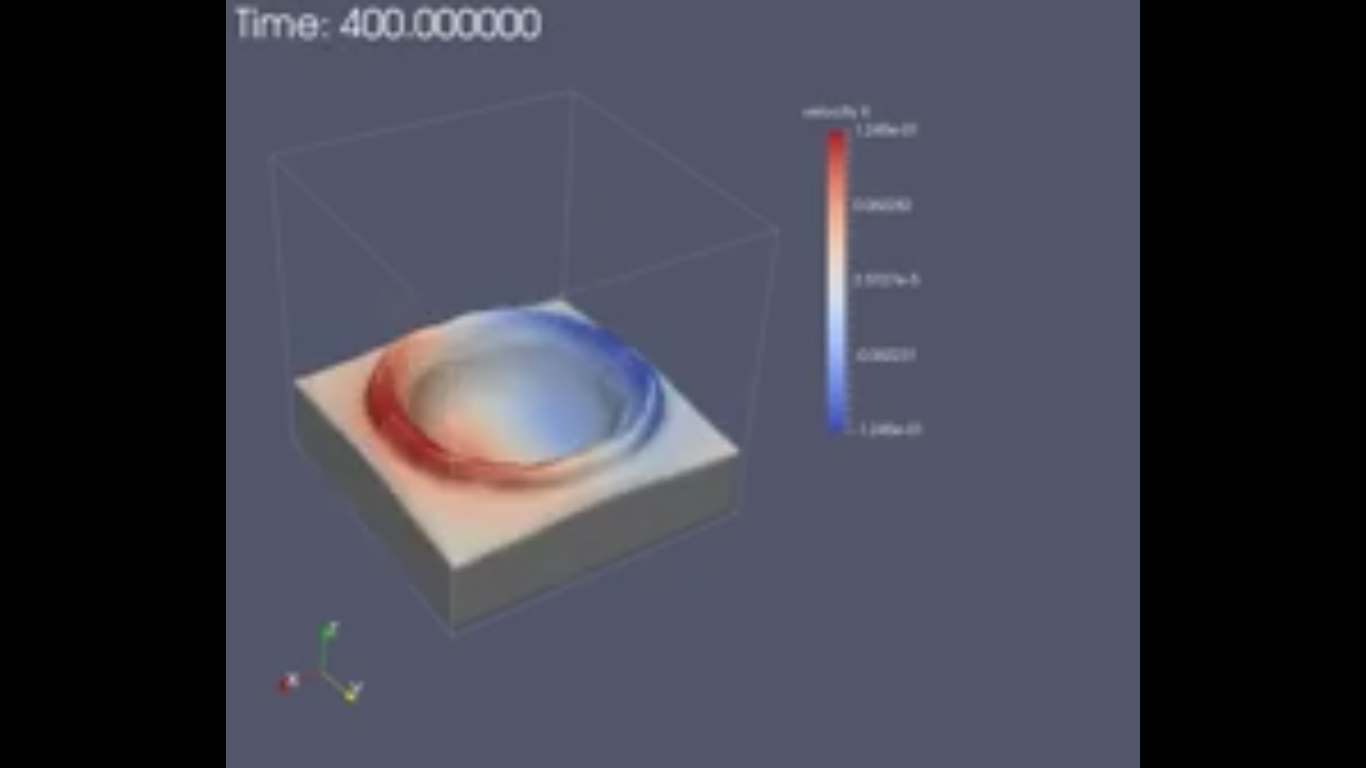
\includegraphics[width=1.0\linewidth]{drop/2.png}
\end{subfigure}
\begin{subfigure}{0.25\textwidth}
  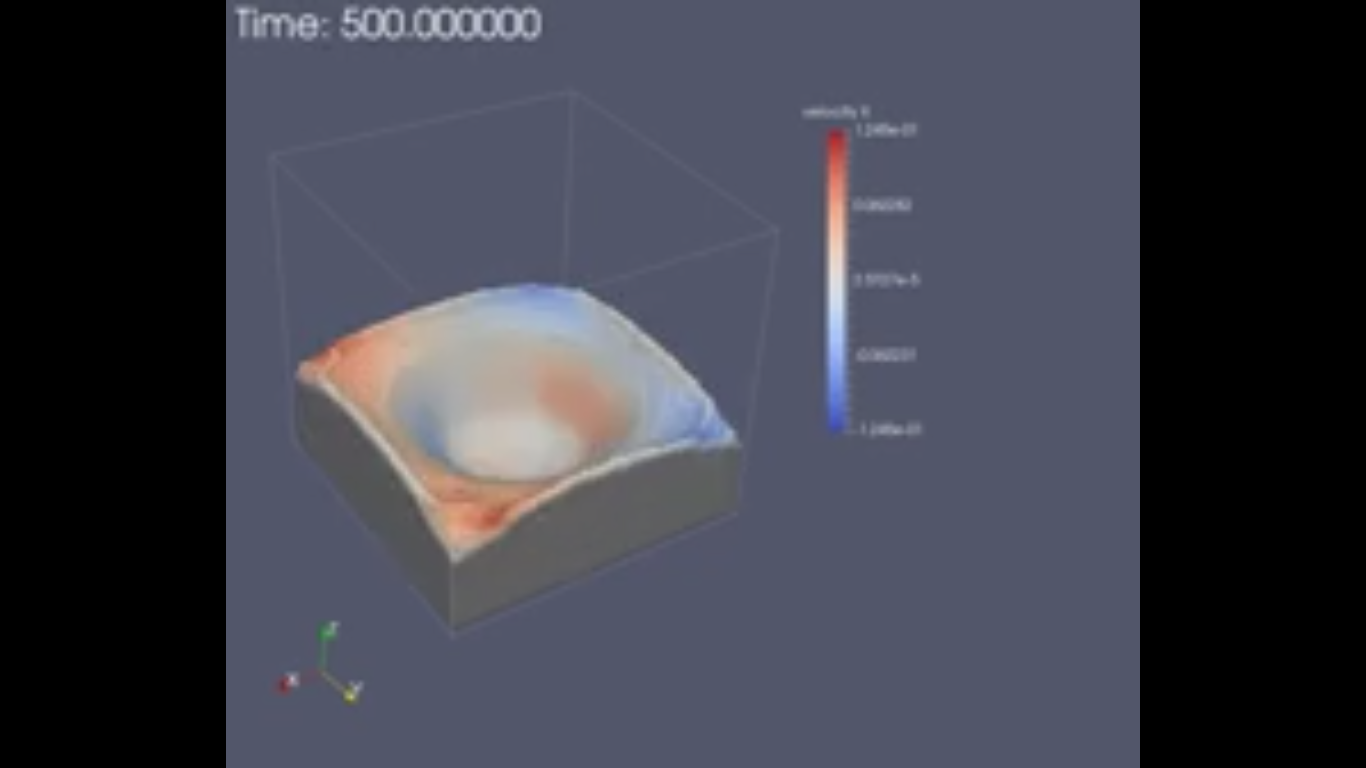
\includegraphics[width=1.0\linewidth]{drop/3.png}
\end{subfigure}
\centering
\begin{subfigure}{0.25\textwidth}
  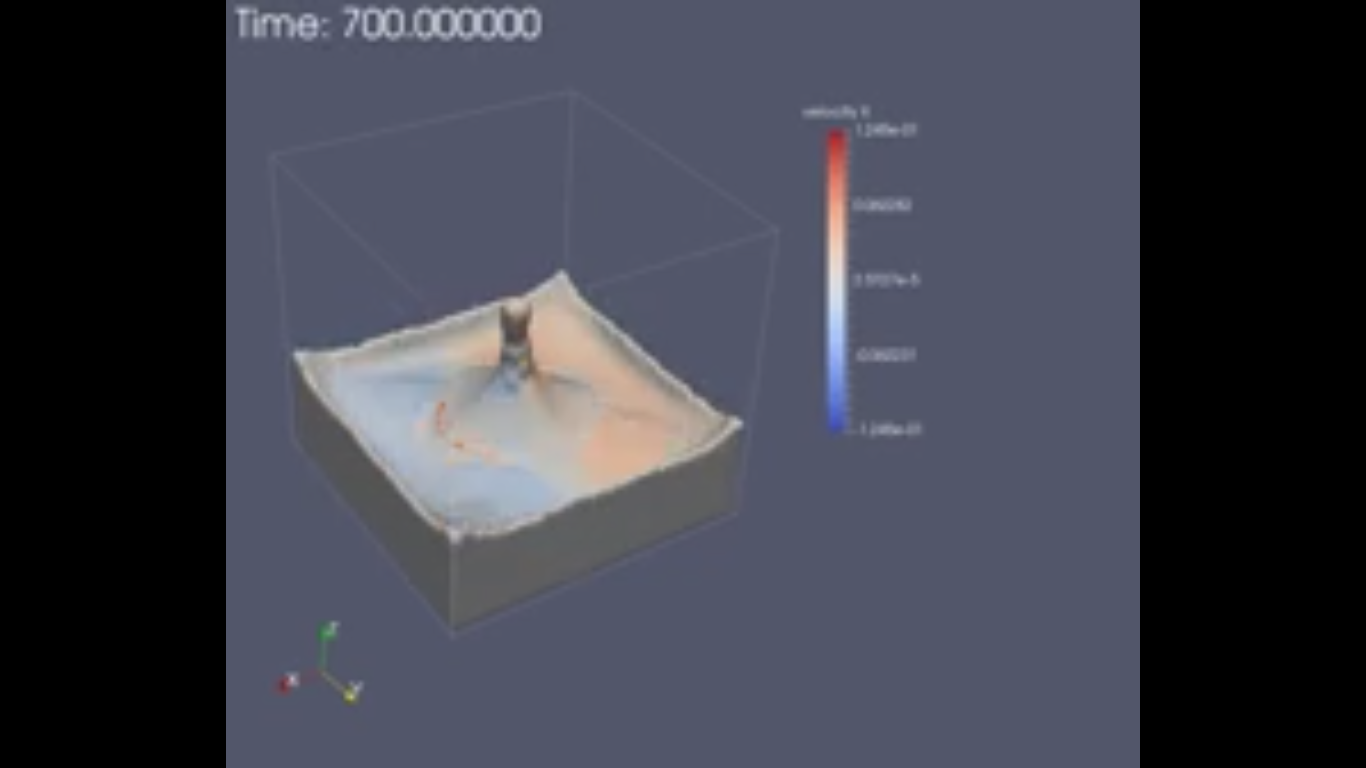
\includegraphics[width=1.0\linewidth]{drop/4.png}
\end{subfigure}%
\begin{subfigure}{0.25\textwidth}
  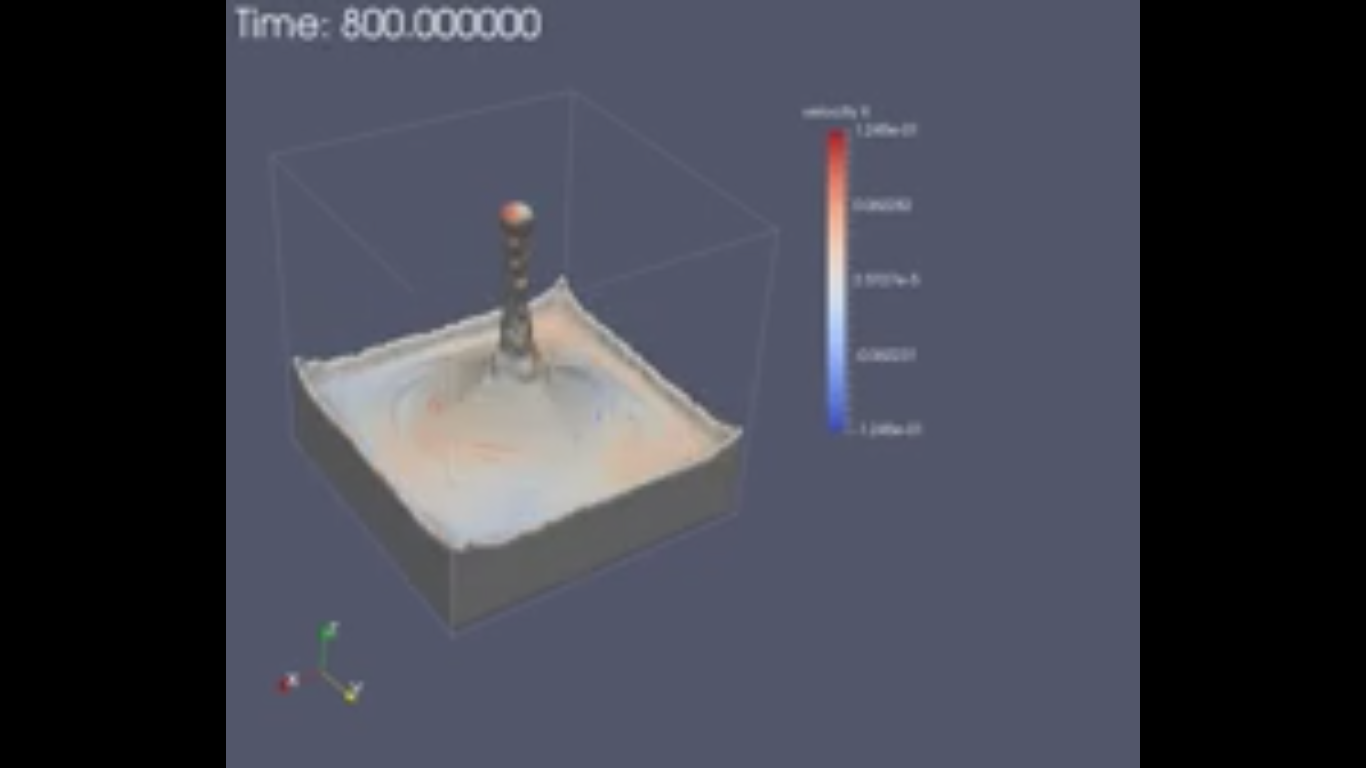
\includegraphics[width=1.0\linewidth]{drop/5.png}
\end{subfigure}
\begin{subfigure}{0.25\textwidth}
  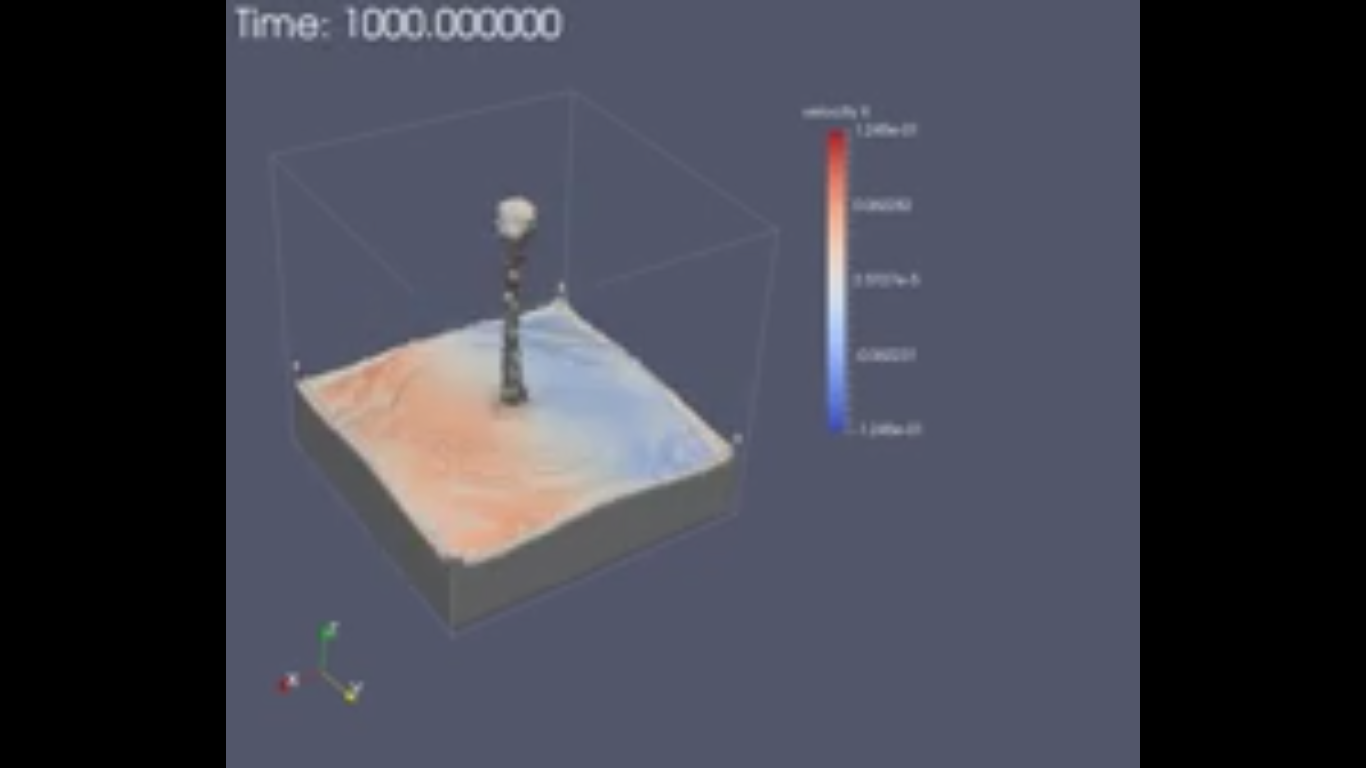
\includegraphics[width=1.0\linewidth]{drop/6.png}
\end{subfigure}
\centering
\begin{subfigure}{0.25\textwidth}
  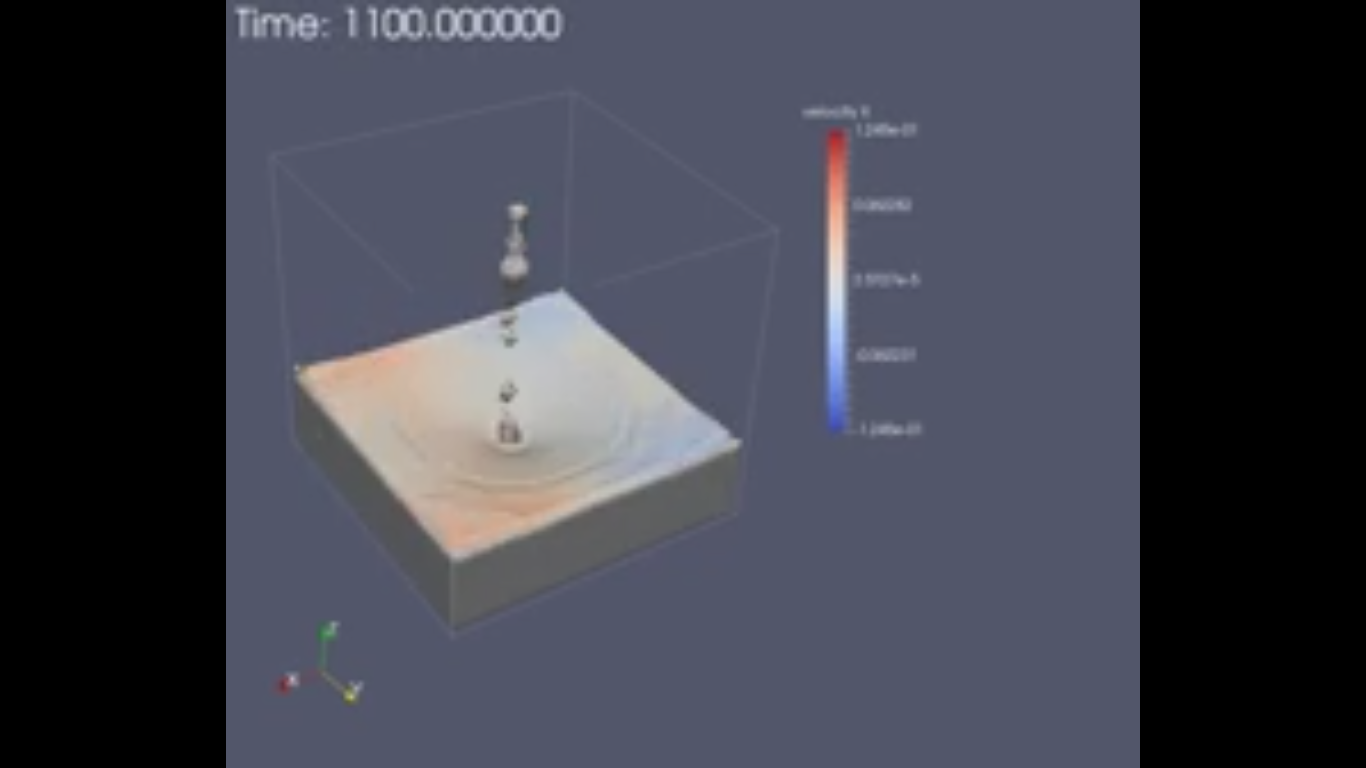
\includegraphics[width=1.0\linewidth]{drop/7.png}
\end{subfigure}%
\begin{subfigure}{0.25\textwidth}
  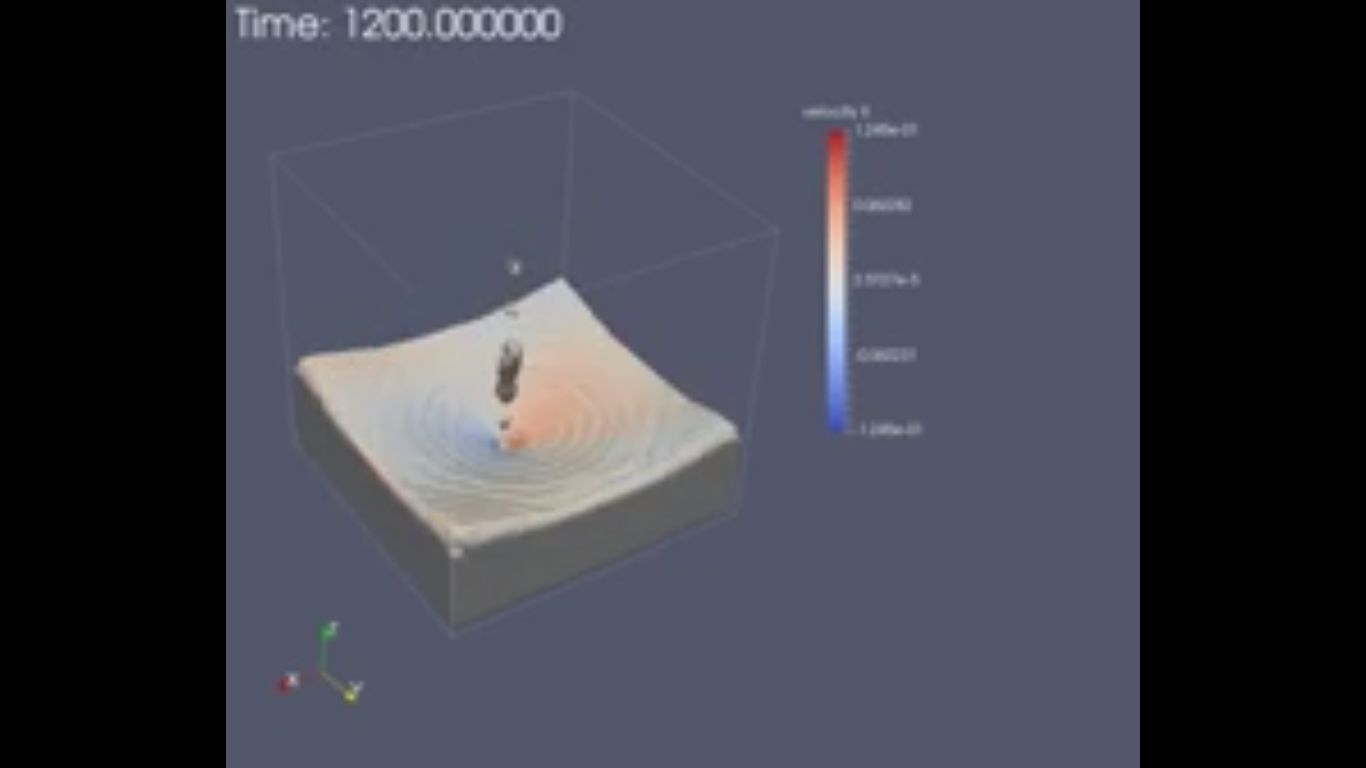
\includegraphics[width=1.0\linewidth]{drop/8.png}
\end{subfigure}
\begin{subfigure}{0.25\textwidth}
  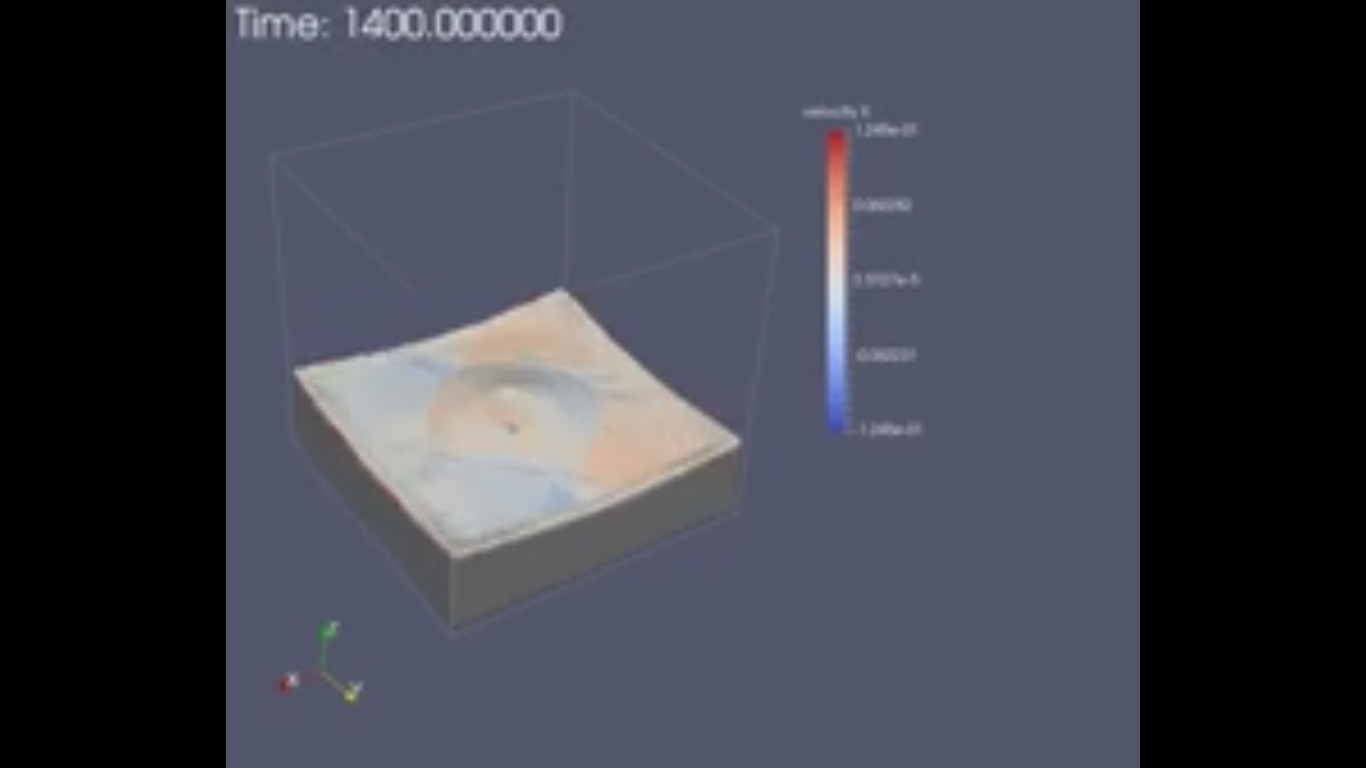
\includegraphics[width=1.0\linewidth]{drop/9.png}
\end{subfigure}
\caption{Falling Drop}
\label{fig:drop}
\end{figure}

\bibliographystyle{alpha}
\bibliography{refs}

\end{document}\grid



\grid
\grid
